
%% cpe621.tex
%% 2017/07/20
%% by Ashton Johnson 
%% see http://github.com/ashtonchase/portable_impedance_tomograhy
%% for current contact information.
%%
%% This is a skeleton file demonstrating the use of IEEEtran.cls
%% (requires IEEEtran.cls version 1.8b or later) with an IEEE
%% journal paper.
%%
%% Support sites:
%% http://www.michaelshell.org/tex/ieeetran/
%% http://www.ctan.org/pkg/ieeetran
%% and
%% http://www.ieee.org/

%%*************************************************************************
%% Legal Notice:
%% This code is offered as-is without any warranty either expressed or
%% implied; without even the implied warranty of MERCHANTABILITY or
%% FITNESS FOR A PARTICULAR PURPOSE! 
%% User assumes all risk.
%% In no event shall the IEEE or any contributor to this code be liable for
%% any damages or losses, including, but not limited to, incidental,
%% consequential, or any other damages, resulting from the use or misuse
%% of any information contained here.
%%
%% All comments are the opinions of their respective authors and are not
%% necessarily endorsed by the IEEE.
%%
%% This work is distributed under the LaTeX Project Public License (LPPL)
%% ( http://www.latex-project.org/ ) version 1.3, and may be freely used,
%% distributed and modified. A copy of the LPPL, version 1.3, is included
%% in the base LaTeX documentation of all distributions of LaTeX released
%% 2003/12/01 or later.
%% Retain all contribution notices and credits.
%% ** Modified files should be clearly indicated as such, including  **
%% ** renaming them and changing author support contact information. **
%%*************************************************************************


% *** Authors should verify (and, if needed, correct) their LaTeX system  ***
% *** with the testflow diagnostic prior to trusting their LaTeX platform ***
% *** with production work. The IEEE's font choices and paper sizes can   ***
% *** trigger bugs that do not appear when using other class files.       ***
% The testflow support page is at:
% http://www.michaelshell.org/tex/testflow/



%\documentclass[journal]{IEEEtran}
%
% If IEEEtran.cls has not been installed into the LaTeX system files,
% manually specify the path to it like:
 \documentclass[]{IEEEtran}

% Some very useful LaTeX packages include:
% (uncomment the ones you want to load)

% *** MISC UTILITY PACKAGES ***
%
%\usepackage{ifpdf}
% Heiko Oberdiek's ifpdf.sty is very useful if you need conditional
% compilation based on whether the output is pdf or dvi.
% usage:
% \ifpdf
%   pdf code
% \else
%    dvi code
% \fi
% The latest version of ifpdf.sty can be obtained from:
% http://www.ctan.org/pkg/ifpdf
% Also, note that IEEEtran.cls V1.7 and later provides a builtin
% \ifCLASSINFOpdf conditional that works the same way.
% When switching from latex to pdflatex and vice-versa, the compiler may
% have to be run twice to clear warning/error messages.

% *** CITATION PACKAGES ***
%
\usepackage{cite}
% cite.sty was written by Donald Arseneau
% V1.6 and later of IEEEtran pre-defines the format of the cite.sty package
% \cite{} output to follow that of the IEEE. Loading the cite package will
% result in citation numbers being automatically sorted and properly
% "compressed/ranged". e.g., [1], [9], [2], [7], [5], [6] without using
% cite.sty will become [1], [2], [5]--[7], [9] using cite.sty. cite.sty's
% \cite will automatically add leading space, if needed. Use cite.sty's
% noadjust option (cite.sty V3.8 and later) if you want to turn this off
% such as if a citation ever needs to be enclosed in parenthesis.
% cite.sty is already installed on most LaTeX systems. Be sure and use
% version 5.0 (2009-03-20) and later if using hyperref.sty.
% The latest version can be obtained at:
% http://www.ctan.org/pkg/cite
% The documentation is contained in the cite.sty file itself.

% *** GRAPHICS RELATED PACKAGES ***
%
\ifCLASSINFOpdf
   \usepackage{graphicx}
  % declare the path(s) where your graphic files are
%   \graphicspath{{../pdf/}{../jpeg/}}
  % and their extensions so you won't have to specify these with
  % every instance of \includegraphics
   \DeclareGraphicsExtensions{.pdf,.jpeg,.png}
\else
  % or other class option (dvipsone, dvipdf, if not using dvips). graphicx
  % will default to the driver specified in the system graphics.cfg if no
  % driver is specified.
   \usepackage[pdftex]{graphicx}
  % declare the path(s) where your graphic files are
 %  \graphicspath{{../pdf/}}
  % and their extensions so you won't have to specify these with
  % every instance of \includegraphics
%   \DeclareGraphicsExtensions{.eps,.pdf}
\fi
% graphicx was written by David Carlisle and Sebastian Rahtz. It is
% required if you want graphics, photos, etc. graphicx.sty is already
% installed on most LaTeX systems. The latest version and documentation
% can be obtained at: 
% http://www.ctan.org/pkg/graphicx
% Another good source of documentation is "Using Imported Graphics in
% LaTeX2e" by Keith Reckdahl which can be found at:
% http://www.ctan.org/pkg/epslatex
%
% latex, and pdflatex in dvi mode, support graphics in encapsulated
% postscript (.eps) format. pdflatex in pdf mode supports graphics
% in .pdf, .jpeg, .png and .mps (metapost) formats. Users should ensure
% that all non-photo figures use a vector format (.eps, .pdf, .mps) and
% not a bitmapped formats (.jpeg, .png). The IEEE frowns on bitmapped formats
% which can result in "jaggedy"/blurry rendering of lines and letters as
% well as large increases in file sizes.
%
% You can find documentation about the pdfTeX application at:
% http://www.tug.org/applications/pdftex





% *** MATH PACKAGES ***
%
%\usepackage{amsmath}
% A popular package from the American Mathematical Society that provides
% many useful and powerful commands for dealing with mathematics.
%
% Note that the amsmath package sets \interdisplaylinepenalty to 10000
% thus preventing page breaks from occurring within multiline equations. Use:
%\interdisplaylinepenalty=2500
% after loading amsmath to restore such page breaks as IEEEtran.cls normally
% does. amsmath.sty is already installed on most LaTeX systems. The latest
% version and documentation can be obtained at:
% http://www.ctan.org/pkg/amsmath





% *** SPECIALIZED LIST PACKAGES ***
%
%\usepackage{algorithmic}
% algorithmic.sty was written by Peter Williams and Rogerio Brito.
% This package provides an algorithmic environment fo describing algorithms.
% You can use the algorithmic environment in-text or within a figure
% environment to provide for a floating algorithm. Do NOT use the algorithm
% floating environment provided by algorithm.sty (by the same authors) or
% algorithm2e.sty (by Christophe Fiorio) as the IEEE does not use dedicated
% algorithm float types and packages that provide these will not provide
% correct IEEE style captions. The latest version and documentation of
% algorithmic.sty can be obtained at:
% http://www.ctan.org/pkg/algorithms
% Also of interest may be the (relatively newer and more customizable)
% algorithmicx.sty package by Szasz Janos:
% http://www.ctan.org/pkg/algorithmicx




% *** ALIGNMENT PACKAGES ***
%
%\usepackage{array}
% Frank Mittelbach's and David Carlisle's array.sty patches and improves
% the standard LaTeX2e array and tabular environments to provide better
% appearance and additional user controls. As the default LaTeX2e table
% generation code is lacking to the point of almost being broken with
% respect to the quality of the end results, all users are strongly
% advised to use an enhanced (at the very least that provided by array.sty)
% set of table tools. array.sty is already installed on most systems. The
% latest version and documentation can be obtained at:
% http://www.ctan.org/pkg/array


% IEEEtran contains the IEEEeqnarray family of commands that can be used to
% generate multiline equations as well as matrices, tables, etc., of high
% quality.




% *** SUBFIGURE PACKAGES ***
%\ifCLASSOPTIONcompsoc
%  \usepackage[caption=false,font=normalsize,labelfont=sf,textfont=sf]{subfig}
%\else
%  \usepackage[caption=false,font=footnotesize]{subfig}
%\fi
% subfig.sty, written by Steven Douglas Cochran, is the modern replacement
% for subfigure.sty, the latter of which is no longer maintained and is
% incompatible with some LaTeX packages including fixltx2e. However,
% subfig.sty requires and automatically loads Axel Sommerfeldt's caption.sty
% which will override IEEEtran.cls' handling of captions and this will result
% in non-IEEE style figure/table captions. To prevent this problem, be sure
% and invoke subfig.sty's "caption=false" package option (available since
% subfig.sty version 1.3, 2005/06/28) as this is will preserve IEEEtran.cls
% handling of captions.
% Note that the Computer Society format requires a larger sans serif font
% than the serif footnote size font used in traditional IEEE formatting
% and thus the need to invoke different subfig.sty package options depending
% on whether compsoc mode has been enabled.
%
% The latest version and documentation of subfig.sty can be obtained at:
% http://www.ctan.org/pkg/subfig




% *** FLOAT PACKAGES ***
%
%\usepackage{fixltx2e}
% fixltx2e, the successor to the earlier fix2col.sty, was written by
% Frank Mittelbach and David Carlisle. This package corrects a few problems
% in the LaTeX2e kernel, the most notable of which is that in current
% LaTeX2e releases, the ordering of single and double column floats is not
% guaranteed to be preserved. Thus, an unpatched LaTeX2e can allow a
% single column figure to be placed prior to an earlier double column
% figure.
% Be aware that LaTeX2e kernels dated 2015 and later have fixltx2e.sty's
% corrections already built into the system in which case a warning will
% be issued if an attempt is made to load fixltx2e.sty as it is no longer
% needed.
% The latest version and documentation can be found at:
% http://www.ctan.org/pkg/fixltx2e


%\usepackage{stfloats}
% stfloats.sty was written by Sigitas Tolusis. This package gives LaTeX2e
% the ability to do double column floats at the bottom of the page as well
% as the top. (e.g., "\begin{figure*}[!b]" is not normally possible in
% LaTeX2e). It also provides a command:
%\fnbelowfloat
% to enable the placement of footnotes below bottom floats (the standard
% LaTeX2e kernel puts them above bottom floats). This is an invasive package
% which rewrites many portions of the LaTeX2e float routines. It may not work
% with other packages that modify the LaTeX2e float routines. The latest
% version and documentation can be obtained at:
% http://www.ctan.org/pkg/stfloats
% Do not use the stfloats baselinefloat ability as the IEEE does not allow
% \baselineskip to stretch. Authors submitting work to the IEEE should note
% that the IEEE rarely uses double column equations and that authors should try
% to avoid such use. Do not be tempted to use the cuted.sty or midfloat.sty
% packages (also by Sigitas Tolusis) as the IEEE does not format its papers in
% such ways.
% Do not attempt to use stfloats with fixltx2e as they are incompatible.
% Instead, use Morten Hogholm'a dblfloatfix which combines the features
% of both fixltx2e and stfloats:
%
% \usepackage{dblfloatfix}
% The latest version can be found at:
% http://www.ctan.org/pkg/dblfloatfix




%\ifCLASSOPTIONcaptionsoff
%  \usepackage[nomarkers]{endfloat}
% \let\MYoriglatexcaption\caption
% \renewcommand{\caption}[2][\relax]{\MYoriglatexcaption[#2]{#2}}
%\fi
% endfloat.sty was written by James Darrell McCauley, Jeff Goldberg and 
% Axel Sommerfeldt. This package may be useful when used in conjunction with 
% IEEEtran.cls'  captionsoff option. Some IEEE journals/societies require that
% submissions have lists of figures/tables at the end of the paper and that
% figures/tables without any captions are placed on a page by themselves at
% the end of the document. If needed, the draftcls IEEEtran class option or
% \CLASSINPUTbaselinestretch interface can be used to increase the line
% spacing as well. Be sure and use the nomarkers option of endfloat to
% prevent endfloat from "marking" where the figures would have been placed
% in the text. The two hack lines of code above are a slight modification of
% that suggested by in the endfloat docs (section 8.4.1) to ensure that
% the full captions always appear in the list of figures/tables - even if
% the user used the short optional argument of \caption[]{}.
% IEEE papers do not typically make use of \caption[]'s optional argument,
% so this should not be an issue. A similar trick can be used to disable
% captions of packages such as subfig.sty that lack options to turn off
% the subcaptions:
% For subfig.sty:
% \let\MYorigsubfloat\subfloat
% \renewcommand{\subfloat}[2][\relax]{\MYorigsubfloat[]{#2}}
% However, the above trick will not work if both optional arguments of
% the \subfloat command are used. Furthermore, there needs to be a
% description of each subfigure *somewhere* and endfloat does not add
% subfigure captions to its list of figures. Thus, the best approach is to
% avoid the use of subfigure captions (many IEEE journals avoid them anyway)
% and instead reference/explain all the subfigures within the main caption.
% The latest version of endfloat.sty and its documentation can obtained at:
% http://www.ctan.org/pkg/endfloat
%
% The IEEEtran \ifCLASSOPTIONcaptionsoff conditional can also be used
% later in the document, say, to conditionally put the References on a 
% page by themselves.




% *** PDF, URL AND HYPERLINK PACKAGES ***
%
\usepackage{url}
% url.sty was written by Donald Arseneau. It provides better support for
% handling and breaking URLs. url.sty is already installed on most LaTeX
% systems. The latest version and documentation can be obtained at:
% http://www.ctan.org/pkg/url
% Basically, \url{my_url_here}.




% *** Do not adjust lengths that control margins, column widths, etc. ***
% *** Do not use packages that alter fonts (such as pslatex).         ***
% There should be no need to do such things with IEEEtran.cls V1.6 and later.
% (Unless specifically asked to do so by the journal or conference you plan
% to submit to, of course. )


% correct bad hyphenation here
\hyphenation{op-tical net-works semi-conduc-tor}


\begin{document}
%
% paper title
% Titles are generally capitalized except for words such as a, an, and, as,
% at, but, by, for, in, nor, of, on, or, the, to and up, which are usually
% not capitalized unless they are the first or last word of the title.
% Linebreaks \\ can be used within to get better formatting as desired.
% Do not put math or special symbols in the title.
\title {A Portable Impedance\\Tomography Platform}

%
%
% author names and IEEE memberships
% note positions of commas and nonbreaking spaces ( ~ ) LaTeX will not break
% a structure at a ~ so this keeps an author's name from being broken across
% two lines.
% use \thanks{} to gain access to the first footnote area
% a separate \thanks must be used for each paragraph as LaTeX2e's \thanks
% was not built to handle multiple paragraphs
%

\author{Ashton Johnson\thanks{Prof. Emil Jovanov with the Department of Electrical and Computer Engineering, University of Alabama in Huntsville, Huntsville, AL 35899}}% <-this % stops a space


% note the % following the last \IEEEmembership and also \thanks - 
% these prevent an unwanted space from occurring between the last author name
% and the end of the author line. i.e., if you had this:
% 
% \author{....lastname \thanks{...} \thanks{...} }
%                     ^------------^------------^----Do not want these spaces!
%
% a space would be appended to the last name and could cause every name on that
% line to be shifted left slightly. This is one of those "LaTeX things". For
% instance, "\textbf{A} \textbf{B}" will typeset as "A B" not "AB". To get
% "AB" then you have to do: "\textbf{A}\textbf{B}"
% \thanks is no different in this regard, so shield the last } of each \thanks
% that ends a line with a % and do not let a space in before the next \thanks.
% Spaces after \IEEEmembership other than the last one are OK (and needed) as
% you are supposed to have spaces between the names. For what it is worth,
% this is a minor point as most people would not even notice if the said evil
% space somehow managed to creep in.



% The paper headers
\markboth{CPE 621, FALL 2017}%
{Shell \MakeLowercase{\textit{Johnson}}: Portable Impedance Tomography Platform}
% The only time the second header will appear is for the odd numbered pages
% after the title page when using the twoside option.
% 
% *** Note that you probably will NOT want to include the author's ***
% *** name in the headers of peer review papers.                   ***
% You can use \ifCLASSOPTIONpeerreview for conditional compilation here if
% you desire.

% If you want to put a publisher's ID mark on the page you can do it like
% this:
%\IEEEpubid{0000--0000/00\$00.00~\copyright~2015 IEEE}
% Remember, if you use this you must call \IEEEpubidadjcol in the second
% column for its text to clear the IEEEpubid mark.

% use for special paper notices
%\IEEEspecialpapernotice{(Invited Paper)}

% make the title area
\maketitle

% As a general rule, do not put math, special symbols or citations
% in the abstract or keywords.
\begin{abstract}
Electrical impedance analysis is a non-invasive technique use for determining the density and composition of various materials. Regarding the human body, one dimensional analysis can determine water content, body fat, and blood glucose measurements. Using multiple electrode sets, we developed a solution to provide two dimensional (2D) tomography imaging. A portable bio-impedance tomography unit is realized using the Analog Devices AD5933 integrated circuit for measuring complex impedance, an analog front end for interfacing to the human body and analog multiplexers. We implement this as a portable device that can be accessed using Bluetooth Low Energy.
\end{abstract}

% Note that keywords are not normally used for peerreview papers.
\begin{IEEEkeywords}
bioimpedance, AD5933, tomography, impedance, Bluetooth, BLE, smartphone, PSoC, Cypress, pmod
\end{IEEEkeywords}



% For peer review papers, you can put extra information on the cover
% page as needed:
% \ifCLASSOPTIONpeerreview
% \begin{center} \bfseries EDICS Category: 3-BBND \end{center}
% \fi
%
% For peerreview papers, this IEEEtran command inserts a page break and
% creates the second title. It will be ignored for other modes.
%\IEEEpeerreviewmaketitle



\section{Introduction}

\IEEEPARstart{T}{he} impedance of an object can provide meaningful insight into the composition of that particular object. 
\newline 
% You must have at least 2 lines in the paragraph with the drop letter
% (should never be an issue)

%\hfill acj
%\hfill October 22, 2017

\section{Project Goals}
The goals of this project to develop a portable solution for impedance measurements. It shall have the following features:
% needed in second column of first page if using \IEEEpubid
%\IEEEpubidadjcol
\begin{itemize}
\item{Single Frequency Impedance Measurement}%TODO determine to to remove colons generated
\item{Frequency Swept Impedance Mesaurement}
\item{Two-dimensional Impedance Measurements}
\item{Portability}
\itme{Bluetooth Connectivity}
\end{itemize}


\section{Impedance Overview}
Impedance can be defined as the effective resistance of an electric circuit or component to alternating current, arising from the combined effects of ohmic resistance and frequency dependent reactance. At a frequency of zero Hertz, the impedance is simply the ohmic resistance. The impedance of a circuit can be though of as complex number, where the real part is the ohmic resistance and the imaginary part is the reactance. Therefore the impedance can be expresses as \[Z=R+jX\]. In application, there are two ideal components that that have purely reactive impedance. That is, the \(R\) is zero; therefore \(Z=jX\). One component is an inductor, whose impedance is expressed as \[Z_L=j\omegaL\] where \(\omega=2*\pi*freq(Hz)\) and L is the inductance in Henries. The other component is a capacitor, whose impedance is expressed as \[Z_C=\frac{1}{j\omegaC}\] where \(\omega=2*\pi*freq(Hz)\) and C is the capacitance in Farads.\newline

\subsection{Applications}
There are numerous applications where impedance can be used an investigative tool. Electrochemical Impedance Spectroscopy is a process that is used to characterize chemical coatings on materials\cite{macdonald_reflections_2006}. Practically, this allows for analysis such as the anodic corrosion of iron in sulfuric acid, the effectiveness of sensitizers in dye-sensitized solar cells\cite{wang_electrochemical_2005}, or monitoring the corrosion of reinforced concrete\cite{ribeiro_use_2015}. \cite{barsoukov_impedance_2005} focuses a great deal on using Impedance Spectroscopy to analyze battery chemical compositions. Impedance Spectroscopy is also widely used on organic matter, specifically on the human body. This is more formally defined as Electrical Bioimpedance Impedance Spectroscopy (BIS), or Bioelectrical Impedance Analysis (BIA). This include the more commonly known Body Composition Measurements such as total body water (TBW) content and body fat estimation. The human body can be generalized in a circuit that has a complex impedance. It is a combination of purely resistance elements, as well as capacitive elements. The exact values of these components are dependent on many factors including electrode placement, water content, salt content, movement and other factors.\cite{lukaski_assessment_1985} performs a thorough characterization of the human body. Impedance Pneuemography use for monitoring an individuals respiration rates and cardiac output\cite{grenvik_impedance_1972},\cite{larsen_impedance_1984},\cite{ernst_impedance_1999}.
\newline
This paper focuses specifically with the two-dimensional (2D) and three-dimensional (3D) application of impedance measurement. This is known at Electrical Impedance Tomography (EIT), and is an imaging technique already in use. This imaging can be performed at a single frequency or across a frequency spectrum. It's worth noting here that EIU is a not a replacement for Magnetic Resonance Imaging (MRI) or X-ray computerize tomography (CT) Scans. This is because unlike a x-ray vector fields in CT scan, the current flowing across the electrodes of a EIT scanner is not fixed in the transverse plane of the measurement electrodes. The results of the EIT scan are more effective the more consistent the composition is as you extend tangentially away from the transverse scan plane. An example of this is the thorax when considering a scan of the lungs, as the lungs are more than an order of magnitude taller than the height of the electrodes place around the thorax. \cite{adler_electrical_2017} thoroughly covers EIT and it's applications, implementation considerations, and image reconstruction. 



\section{Hardware Implementation}
\subsection{Requirements}
The measurement of an unknown impedance is can be found by using a measuring the voltage or current waveforms at two different points in the circuit, shown in Fig~\ref{fig:zun}\cite{noauthor_oscilloscope_nodate}. The magnitude and angle of the impedance of an unknown object at a given frequency can be expressed as

\begin{figure} %reference https://en.wikibooks.org/wiki/LaTeX/Floats,_Figures_and_Captions for [!h] options on placing the figures
\centering
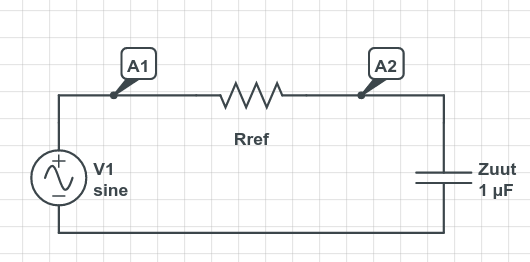
\includegraphics[width=5cm ]{./graphics/zun.png}
\centering
\caption{Circuit for measuring unknown impedance}
\label{fig:zun}
\end{figure}


\[Z_{uut}=\frac{V_{A2}R_{ref}}{\sqrt{V^2_{A1}-2V_{A1}V_{A2}cos\theta+V^2_{A2}}}\]
\newline
\[\alpha_{uut}=\theta-tan^{-1}\frac{-V_{A2}sin\theta}{V_{A1}-V_{A2}cos\theta} \]
where \(\theta\) is the phase difference between measured voltage at A2 relative to A1.
\newline
Another method of determining the impedance is performing a discrete Fourier transform (DFT) on the sampled data of a sine wave passed though the circuit.
\[X(f)=\sum_{n=0}^{N}(x(n)(cos(n)-jsin(n)))\]
where \(X(f)\) is expressed as a complex number \(R+jX\),\(x(n)\)is the resulting signal is ADC sampled waveform that has passed through the unknown impedance. \(cos(n)\) and \(sin(n)\) are from these sourcing waveform passing being passed into the unknown impedance. The magnitude is defined as \(\sqrt{R^2+X^2}\) and the phase is defined as \(tan^{-1}(Z/R)\times\frac{180\textdegree}{\pi}\) in degrees\cite{noauthor_ad5933_nodate}.


\subsection{AD5933}
Analog Devices has introduced a AD5933 integrated circuit (IC) to a monolithic platform for impedance measurement. It is a 1 Megasample per second, 12-Bit Impedance Converter\cite{noauthor_ad5933_nodate}. The response signal from the impedance is sampled by the on-board ADC and a discrete Fourier transform (DFT) is processed by an on-board DSP engine. The DFT algorithm returns a real (R) and imaginary (I) data-word at each output frequency. Once calibrated, the magnitude of the impedance and relative phase of the impedance at each frequency point along the sweep is easily calculated. This is done off chip using the real and imaginary register contents, which can be read from the serial Inter-Integrated Circuit (I2C) interface.\newline
The AD5933 has been evaluated as a suitable platform for BIA\cite{breniuc_wearable_2014},\cite{ferreira_ad5933-based_2011},\cite{harder_smart_2016},\cite{bakr_aging_2016},\cite{pliquett_interfacing_2012}. The analog interface to the unit-under-test (UUT) is not design specific; is a simple voltage digital-to-analog converter (DAC) that drives a single-ended voltage-mode analog-to-digital converter (ADC). For bioimpedance applications, it is important to have a constant current amplitude over the frequency range of interest to ensure accurate measurements\cite{bertemes-filho_mirrored_2012},\cite{seoane_analog_2008},\cite{pliquett_interfacing_2012},\cite{bera_battery-based_2013}. Additionally, it is also important to not exceed safe current levels passing though the human body as defined in IEC60601-1\cite{noauthor_iec_nodate}. This limit is defined as the Patient Auxiliary Current. For DC current, this is limited to 0.05 miliAmperes. For AC current, this is limited to 0.5 miliAmperes. Using a voltage controlled current source, we can precisely control the current flowing through the test subject. 

\subsection{Analog Front End}

\begin{figure} %reference https://en.wikibooks.org/wiki/LaTeX/Floats,_Figures_and_Captions for [!h] options on placing the figures
\centering
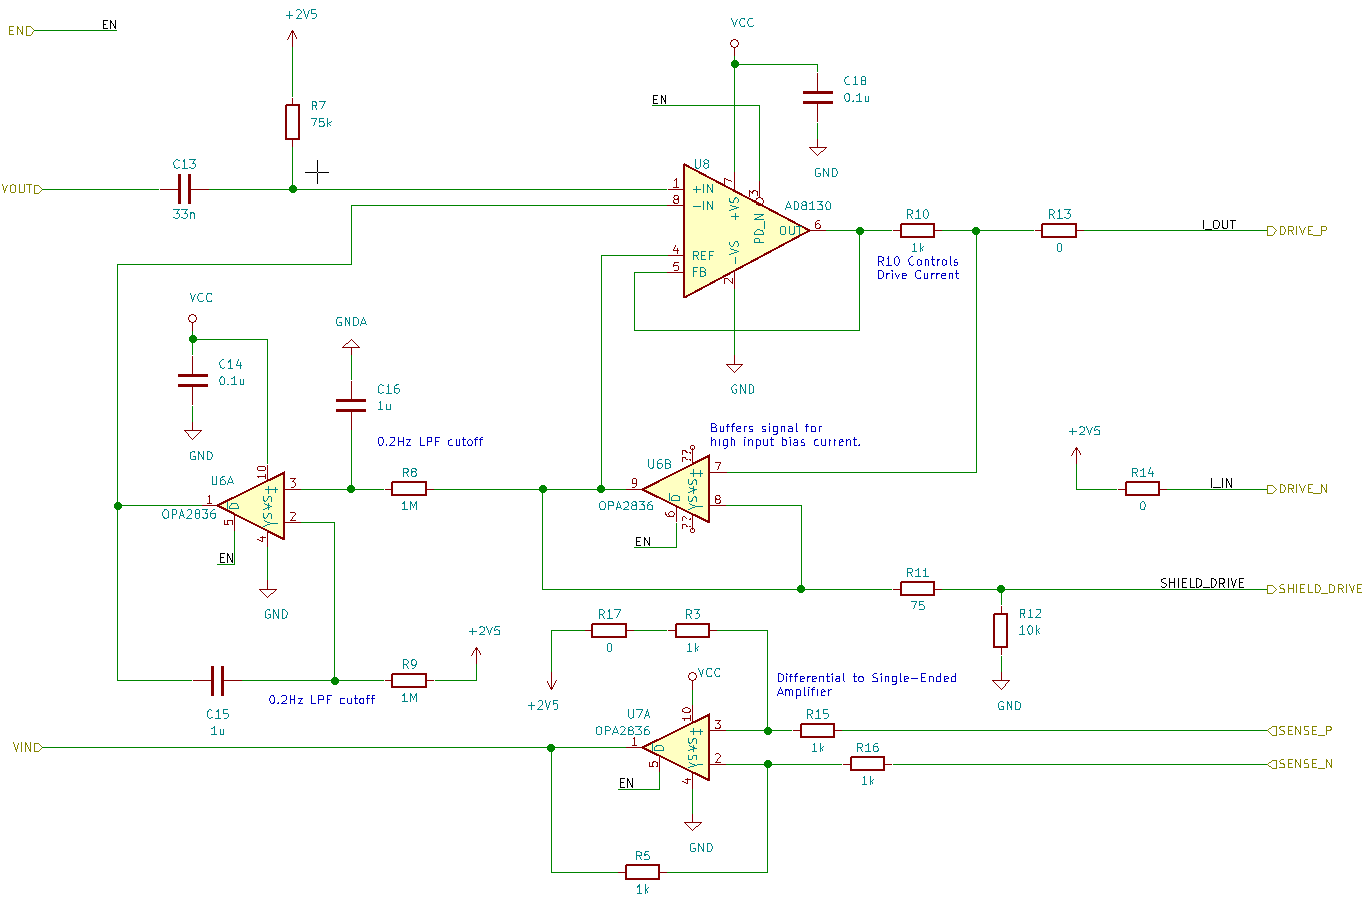
\includegraphics[width=9cm ]{./graphics/front_end.png}
\centering
\caption{Analog Front End}
\label{fig:front_end}
\end{figure}


To accommodate the aforementioned limitations of the AD5933, we implemented a voltage-controlled current source for providing the stimulus the UUT. We also provided a differential input so that the resulting voltage is measured between two electrodes. Differential measurements should eliminate any common mode interference present on the electrodes. The analog front end is based the design described in \cite{harder_smart_2016}. The design shown in In Fig~\ref{fig:front_end} uses an Analog Devices AD8130 differential receiver amplifier\cite{noauthor_ad8130_nodate} as a wide-band voltage controlled current source.

\subsubsection{Electrode Multiplexing}
The AD5933 Impedance analyzer using the analog front end allows for taking measurements across 4 electrodes; two for the excitation and two for the sensing. Spatially, this allows only for a one-dimensional (1D) measurement. For tomography applications, driving one pair of electrodes and sensing on different electrodes is required. \cite{hua_using_1993},\cite{dimas_development_2017},\cite{wang_electrical_nodate}, \cite{vilchez-monge_image_2017} have demonstrated implementations. This allows for a two-dimensional (2D) dataset. For a set of N electrodes, in our case 4 sets, the number of measurements we can have is defined as \[Measurement_{Combinations}=\sum_{i=1}^{i=N-1}i\]. Therefore for 4 sets of sense electrodes, we will have 6 different measurements. These can be shown in the Fig~\ref{fig:combo4}

\begin{figure} %reference https://en.wikibooks.org/wiki/LaTeX/Floats,_Figures_and_Captions for [!h] options on placing the figures
\centering
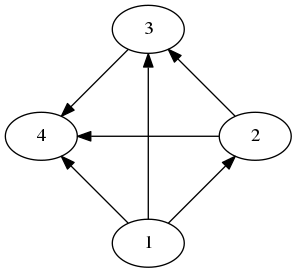
\includegraphics[width=5cm ]{./graphics/combo4.png}
\centering
\caption{Electrode Combinations}
\label{fig:combo4}
\end{figure}

For this design, we not only multiplexed the voltage sense electrodes, but also the current drive electrodes. This means we have \[\sum_{i=1}^{i=N-1}i\times\sum_{i=1}^{i=N-1}i=6\times6=36\]
different combinations of measurements we can collect.

The multiplexing is realized using two Analog Devices AD1209 analog multiplexers. This devices is a differential 4-to-1 multiplexer. This allows us to switch both the drive and the sense simultaneously. In hindsight, this is a design limitation. This actually brings the number of combinations back down to 6, as the voltage can only be sensed on the same channels as the drive.


\begin{figure} %reference https://en.wikibooks.org/wiki/LaTeX/Floats,_Figures_and_Captions for [!h] options on placing the figures
\centering
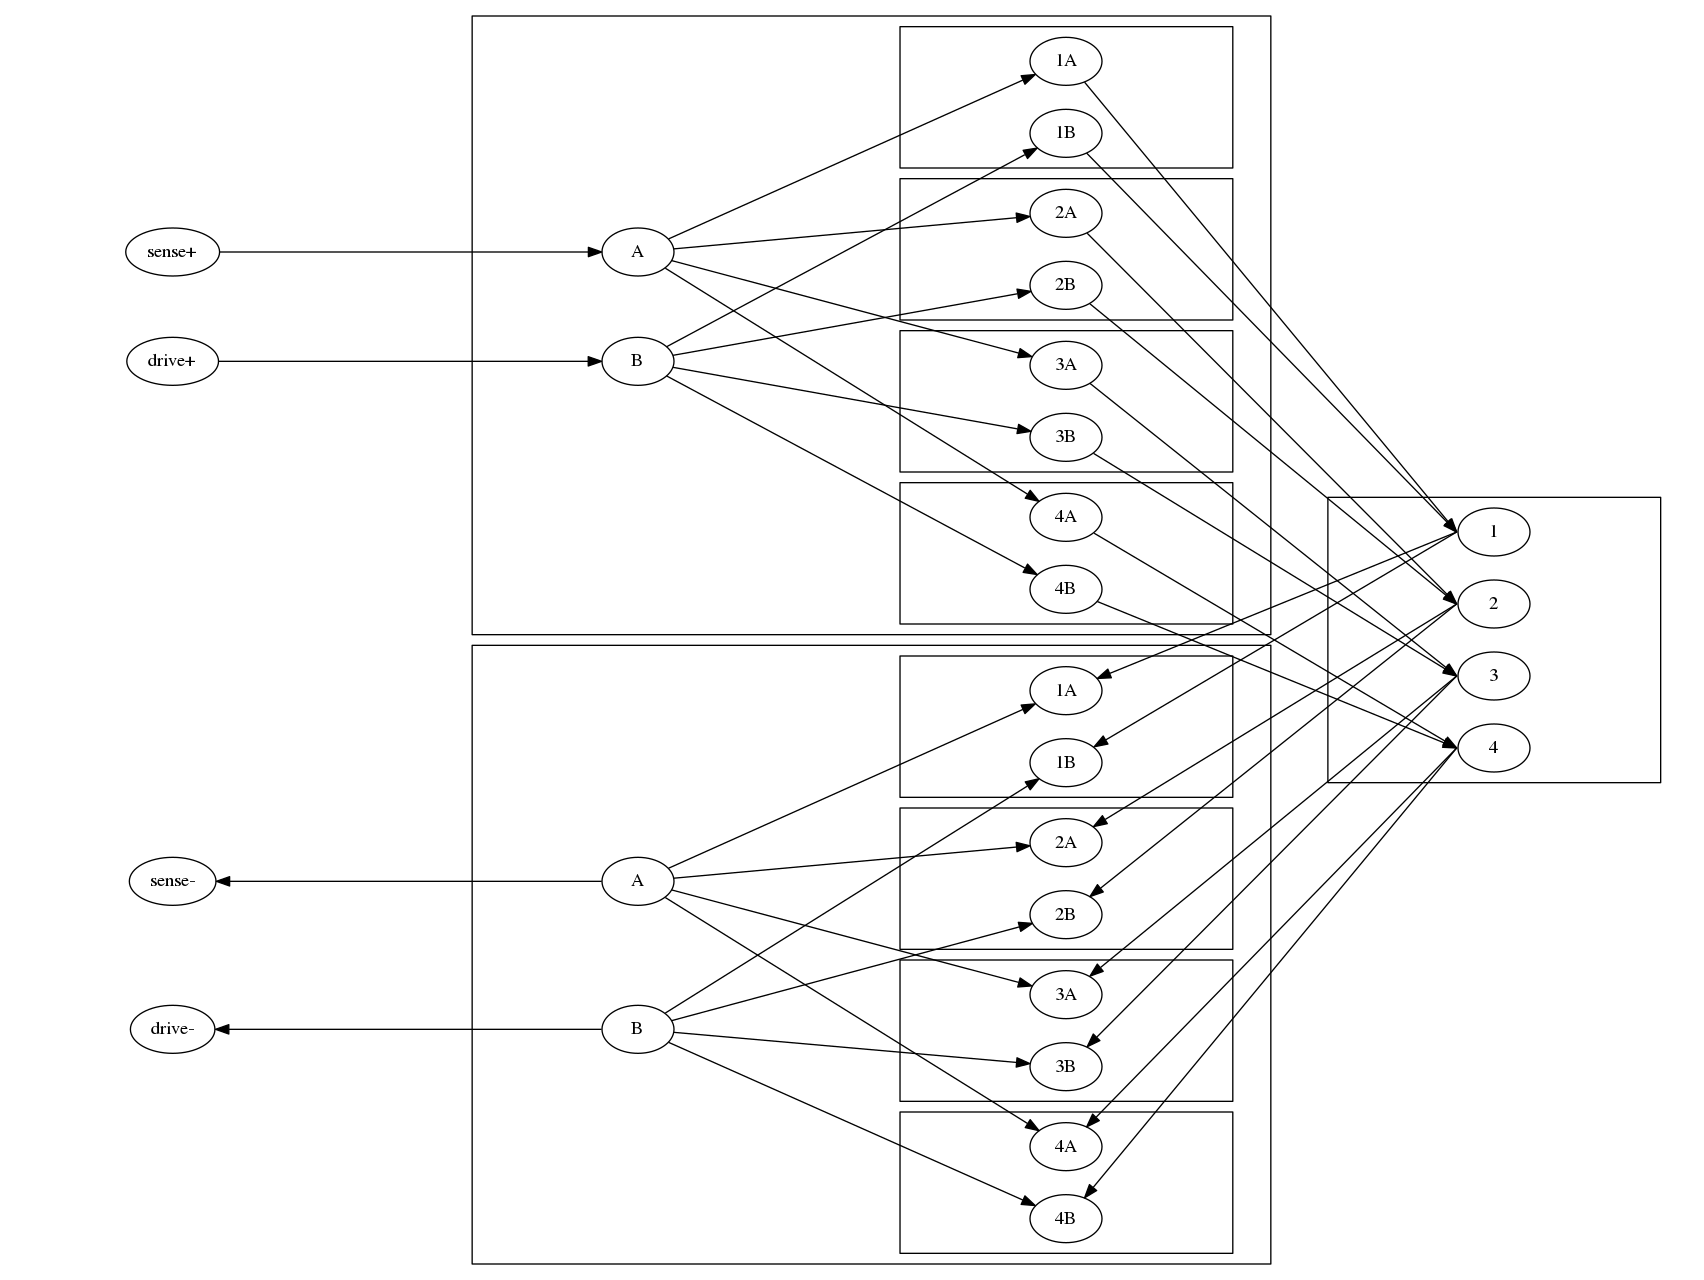
\includegraphics[width=10cm ]{./graphics/mux.png}
\centering
\caption{Electrode Mux Configuration}
\label{fig:mux}
\end{figure}


\subsubsection{Device Controller}
The Cypress CY8CKIT-142 Module. This module is provided as a part of a Bluetooth Low Energy development kit.

\section{Software Implementation}
\subsection {Device States}


\subsection{Communication}


\begin{figure} %reference https://en.wikibooks.org/wiki/LaTeX/Floats,_Figures_and_Captions for [!h] options on placing the figures
\centering
\includegraphics[width=9cm ]{./graphics/zynq_w_gpio.png}
\centering
\caption{Design with GPIO peripheral.}
\label{fig:gpio}
\end{figure}

In Fig~\ref{fig:gpio}, 

\tt{
class DefaultFPGARoccConfig \newline
class DefaultFPGA32KBL2Config \newline
class DefaultFPGA256KBL2Config \newline
class DefaultFPGADualCoreConfig}\rm{}



% An example of a floating figure using the graphicx package.
% Note that \label must occur AFTER (or within) \caption.
% For figures, \caption should occur after the \includegraphics.
% Note that IEEEtran v1.7 and later has special internal code that
% is designed to preserve the operation of \label within \caption
% even when the captionsoff option is in effect. However, because
% of issues like this, it may be the safest practice to put all your
% \label just after \caption rather than within \caption{}.
%
% Reminder: the "draftcls" or "draftclsnofoot", not "draft", class
% option should be used if it is desired that the figures are to be
% displayed while in draft mode.
%
%\begin{figure}[!t]
%\centering
%\includegraphics[width=2.5in]{myfigure}
% where an .eps filename suffix will be assumed under latex, 
% and a .pdf suffix will be assumed for pdflatex; or what has been declared
% via \DeclareGraphicsExtensions.
%\caption{Simulation results for the network.}
%\label{fig_sim}
%\end{figure}

% Note that the IEEE typically puts floats only at the top, even when this
% results in a large percentage of a column being occupied by floats.


% An example of a double column floating figure using two subfigures.
% (The subfig.sty package must be loaded for this to work.)
% The subfigure \label commands are set within each subfloat command,
% and the \label for the overall figure must come after \caption.
% \hfil is used as a separator to get equal spacing.
% Watch out that the combined width of all the subfigures on a 
% line do not exceed the text width or a line break will occur.
%
%\begin{figure*}[!t]
%\centering
%\subfloat[Case I]{\includegraphics[width=2.5in]{box}%
%\label{fig_first_case}}
%\hfil
%\subfloat[Case II]{\includegraphics[width=2.5in]{box}%
%\label{fig_second_case}}
%\caption{Simulation results for the network.}
%\label{fig_sim}
%\end{figure*}
%
% Note that often IEEE papers with subfigures do not employ subfigure
% captions (using the optional argument to \subfloat[]), but instead will
% reference/describe all of them (a), (b), etc., within the main caption.
% Be aware that for subfig.sty to generate the (a), (b), etc., subfigure
% labels, the optional argument to \subfloat must be present. If a
% subcaption is not desired, just leave its contents blank,
% e.g., \subfloat[].


% An example of a floating table. Note that, for IEEE style tables, the
% \caption command should come BEFORE the table and, given that table
% captions serve much like titles, are usually capitalized except for words
% such as a, an, and, as, at, but, by, for, in, nor, of, on, or, the, to
% and up, which are usually not capitalized unless they are the first or
% last word of the caption. Table text will default to \footnotesize as
% the IEEE normally uses this smaller font for tables.
% The \label must come after \caption as always.
%
%\begin{table}[!t]
%% increase table row spacing, adjust to taste
%\renewcommand{\arraystretch}{1.3}
% if using array.sty, it might be a good idea to tweak the value of
% \extrarowheight as needed to properly center the text within the cells
%\caption{An Example of a Table}
%\label{table_example}
%\centering
%% Some packages, such as MDW tools, offer better commands for making tables
%% than the plain LaTeX2e tabular which is used here.
%\begin{tabular}{|c||c|}
%\hline
%One & Two\\
%\hline
%Three & Four\\
%\hline
%\end{tabular}
%\end{table}


% Note that the IEEE does not put floats in the very first column
% - or typically anywhere on the first page for that matter. Also,
% in-text middle ("here") positioning is typically not used, but it
% is allowed and encouraged for Computer Society conferences (but
% not Computer Society journals). Most IEEE journals/conferences use
% top floats exclusively. 
% Note that, LaTeX2e, unlike IEEE journals/conferences, places
% footnotes above bottom floats. This can be corrected via the
% \fnbelowfloat command of the stfloats package.

\section{Conclusion}
RISC-V is an open ISA designed to break open the world of computer architecture. It is making the push to be the first successful open ISA. The ISA is surrounded by many advantages including a software toolchain and a core design tool to generate inexpensive and reliable hardware. This paper documents our investigation into this ISA and its supporting tools. During the course of the paper we have discussed how we tested these tools utilizing the existing documentation from UC Berkeley for the purpose of improving upon it and understanding RISC-V.

We were able to load and test the pre-built designs in their repositories as well as complete their examples. We were also able to learn about the Rocket Chip generator tool and Chisel, its supporting language. Using these we were able to build a basic rocket core from source. Also using the generator, we made modifications to the core design and configuration and synthesized these cores. We also investigated adding a coprocessor (called a RoCC) and how to add it to a core design. We were able to synthesize this as well. 

We had a few failures along the way. Many of these were due to the state of the repositories being in flux or due to venturing into underdocumented or undocumented pieces of the Rocket Chip generator and RISC-V. We believe that these failures can bring to light information that needs future investigation and documentation. 

It is these authors opinion that RISC-V is poised for success. It is at a critical time in which it is being presented to the world, picked apart, and tested. As such we feel that researching and understanding the ISA and the tools that have been created to support it will help expand it use and usability.

% if have a single appendix:
%\appendix[Proof of the Zonklar Equations]
% or
%\appendix  % for no appendix heading
% do not use \section anymore after \appendix, only \section*
% is possibly needed

% use appendices with more than one appendix
% then use \section to start each appendix
% you must declare a \section before using any
% \subsection or using \label (\appendices by itself
% starts a section numbered zero.)
%
\appendix{Source Material}
All source material for this project is provided under the MIT license and is available at \url{https://github.com/ashtonchase/portable_impedance_tomography} . 

% use section* for acknowledgment
\section*{Acknowledgment}
TBD


% Can use something like this to put references on a page
% by themselves when using endfloat and the captionsoff option.
\ifCLASSOPTIONcaptionsoff
  \newpage
\fi



% trigger a \newpage just before the given reference
% number - used to balance the columns on the last page
% adjust value as needed - may need to be readjusted if
% the document is modified later
%\IEEEtriggeratref{8}
% The "triggered" command can be changed if desired:
%\IEEEtriggercmd{\enlargethispage{-5in}}

% references section

% can use a bibliography generated by BibTeX as a .bbl file
% BibTeX documentation can be easily obtained at:
% http://mirror.ctan.org/biblio/bibtex/contrib/doc/
% The IEEEtran BibTeX style support page is at:
% http://www.michaelshell.org/tex/ieeetran/bibtex/
\bibliographystyle{IEEEtran}
% argument is your BibTeX string definitions and bibliography database(s)
\bibliography{report}
%
% <OR> manually copy in the resultant .bbl file
% set second argument of \begin to the number of references
% (used to reserve space for the reference number labels box)
%\begin{thebibliography}{1}
 
%\bibitem{Asanović:EECS-2016-17}
 
%\end{thebibliography}

% biography section
% 
% If you have an EPS/PDF photo (graphicx package needed) extra braces are
% needed around the contents of the optional argument to biography to prevent
% the LaTeX parser from getting confused when it sees the complicated
% \includegraphics command within an optional argument. (You could create
% your own custom macro containing the \includegraphics command to make things
% simpler here.)
%\begin{IEEEbiography}[{\includegraphics[width=1in,height=1.25in,clip,keepaspectratio]{mshell}}]{Michael Shell}
% or if you just want to reserve a space for a photo:

% if you will not have a photo at all:
\begin{IEEEbiographynophoto}{Ashton Johnson}
 received his B.E. degree in wireless engineering from Auburn University in 2011. He is currently seeking his Master's degree in computer engineering at the University of Alabama in Huntsville. He current works as an electrical engineer at Dynetics, Inc. in Huntsville. 
\end{IEEEbiographynophoto}

% insert where needed to balance the two columns on the last page with
% biographies
%\newpage

% You can push biographies down or up by placing
% a \vfill before or after them. The appropriate
% use of \vfill depends on what kind of text is
% on the last page and whether or not the columns
% are being equalized.

%\vfill

% Can be used to pull up biographies so that the bottom of the last one
% is flush with the other column.
%\enlargethispage{-5in}



% that's all folks
\end{document}



